
% JuliaCon proceedings template
\documentclass{juliacon}
\setcounter{page}{1}
\usepackage{graphicx}

\hypersetup{colorlinks=true}
\begin{document}

% **************GENERATED FILE, DO NOT EDIT**************

\title{Interoperating Deep Learning models with ONNX.jl}

\author[1]{Ayush Shridhar}
\author[2]{Phil Tomson}
\author[3]{Mike Innes}

\affil[1]{International Institute of Information Technology, Bhubaneswar, India}
\affil[2]{Unaffiliated}
\affil[3]{Julia Computing, Inc.}

\keywords{Julia, Machine Learning, Deep Learning, Transfer Learning}

\hypersetup{
pdftitle = {Interoperating Deep Learning models with ONNX.jl},
pdfsubject = {JuliaCon 2019 Proceedings},
pdfauthor = {Ayush Shridhar, Phil Tomson, Mike Innes},
pdfkeywords = {Julia, Machine Learning, Deep Learning, Transfer Learning},
}

\maketitle

\begin{abstract}

Flux \cite{innes:2018} is a machine learning framework, written using the numerical computing
language Julia\cite{bezanson2017julia}. The framework makes writing layers as simple as
writing mathematical formulae, and it's advanced AD,
Zygote \cite{DBLP:journals/corr/abs-1810-07951} , applies automatic differentiation (AD) to
calculate derivatives and train the model. It makes heavy use of Julia's language and
compiler features to carry out code analysis and make optimisations.  For example, Julia's
GPU compilation support \cite{besard:2017} can be used to JIT-compile custom GPU kernels for
model layers \cite{CuArrays.jl}. Flux also supports a number of a hardware options, from CPUs,
GPUs and even TPUs via XLA.jl, that compiles Julia code to XLA: an advanced compiler for
linear algebra that is capable of greatly optimizing speed and memory usage in large
deep learning models. 

ONNX.jl is an Open Neural Network Exchange backend for the Flux.jl deep learning framework.
ONNX.jl supports directly importing high quality ONNX standard models into Flux, thus saving
time and reducing the need for additional computation resources. This paper aims at introducing 
ONNX.jl and explaining how it fits into the bigger picture: How we can use the Julia Language, 
specifically Flux.jl and ONNX.jl as a starting for high quality transfer learning of large deep
learning models.

\end{abstract}

\section{Introduction}

The Julia language was introduced to solve the two language problem: In simple words, languages that
are simple to write (high-level) are very slow but those which are difficult to use (low-level) are
way faster. This is because most of the high-level languages weren't written to process a large 
amount of data. Thus engineers, researchers and developers have a hard time developing a lot of 
high performance languages. At the moment, the common protocol is to write the core of the software
in a low-level language (C/C++/Fortran) and wrap it in a high-level language (Python). This results
in optimized performance and ease of use. The Julia language aims to make best of both worlds. It 
provides a high level syntax but manages to perform as fast as C (sometimes even faster).  

Flux.jl is a library for implementing machine learning models, written completely in the Julia
programming language. At the heart of Flux.jl lies Zygote.jl: A source-to-source automatic
differentiation (AD) library that makes complete use of the Julia language compiler to generate
backward pass during training phase of a neural network, with complete support for control flow,
recursion, closures and data structures.  
Implementing models in Flux.jl is as simple as writing regular Julia code. Implementing models
is as simple as writing the formulae for those, and Zygote.jl will compute the derivatives 
seamlessly.  

Flux.jl also provides support for other hardware options using external packages such as CuArrays.jl
and CLArrays.jl. CuArrays is written completely in Julia, making implementing GPU kernels very simple.
Making a model run on GPU can be done in a hassle-free manner: It is as simple as calling a few functions
to transfer data to GPU. Flux.jl also has support for running models on Google's Tensor Processing
Unit (TPU). TPUs help in very fast linear algebra computation. Running Flux models on TPUs is possible
through XLA.jl that compiles Julia code to XLA.  

The FluxML ecosystem provides a number of supporting packages that provide additional functionalities , some of them being (apart from the aforementioned Flux.jl, Zygote.jl and XLA.jl);

\begin{itemize}
    \item ONNX.jl : Open Neural Network eXchange backend for Flux.jl
    \item Metalhead.jl \cite{Metalhead.jl}: Simple plug and play pretrained Flux.jl computer vision models.
    \item Torch.jl \cite{Torch.jl}: This package aims at exposing Torch.tensor types in Julia.
    \item IRTools.jl \cite{IRTools.jl} : Provides an IR format that is easy to manipulate.
    \item FluxJS.jl \cite{FluxJS.jl} : Runs Flux models in the browser, via tensorflow.js
    \item model-zoo \cite{model-zoo}: Collection of implementation of various Flux deep learning models.
\end{itemize}

\section{Open Neural Network eXchange (ONNX)}
Open Neural Network Exchange (ONNX) \cite{bai2019} is an open ecosystem that empowers AI developers to
choose the right tools as their project evolves. ONNX provides an open source format for AI
models, both deep learning and traditional machine learning. ONNX defines the computation graph for a deep learning model along with various operators used in the model.
It provides a set of specifications to convert a model to a basic ONNX format, and
another set of specifications to get the model back from this ONNX form.   At a high
level, ONNX is designed to allow framework inter-operability. There are many excellent
machine learning libraries in various languages : PyTorch \cite{bai2019} , TensorFlow \cite{abadi2016tensorflow} , MXNet \cite{chen2015mxnet} , and Caffe \cite{jia2014caffe} are
just a few that have become very popular in recent years, but there are many others as well.
Machine learning models can be converted to a serialized ONNX format which can then be run
on a number devices. ONNX Runtime is an inference engine written in C++ framework used to 
deploy ONNX format models into production. It works on diverse hardware and support both
deep learning as well as traditional machine learning models.

\subsection{Where does ONNX come in?}
ONNX is a format for representing deep learning models, which can be further run on numerous devices
without worrying much about the implementation. This helps researchers, developers and engineer to
focus on the problem in hand without worrying much about the peripherals, such as the framework
to use, the ability to run a model trained using this particular framework on specialized hardware.
ONNX is is usable anywhere from small mobile devices to large server farms, across chipsets and vendors,
and with extensive runtimes and tools support. ONNX reduces the friction of moving trained AI
models among your favorite tools and frameworks and platforms. A simple example of how ONNX is ideal
for ML is the case when large deep learning models need to be deployed.     Consider 
the simple case of deploying a Deep Learning model to an iOS application. This particular model can 
be implemented in any framework : TensorFlow, PyTorch, MXNet just to name a few. However, iOS 
applications expect to use CoreML inside the application. Up until now, developers have been porting
large models to different frameworks,
which is a waste of time and energy, better spent somewhere else. This is also retraining the entire model from scratch, which isn't efficient. This makes the entire process cumbersome and impractical. ONNX exists to solve this very problem : By connecting the common dots from
different frameworks, ONNX makes it possible to express a model of type A to type B, thus saving time and the need to train the model again.  

\section{ONNX backend in Julia}

ONNX.jl is an ONNX backend written in Julia for the Flux.jl machine learning framework. It can be
used for high-quality inference of pretrained ONNX format machine learning models. At the heart of it, ONNX.jl solves a compiler problem by dealing with intermediate code representations to generate readable graphs. While doing this, ONNX operators are mapped to corresponding Flux layers, thus tracing out the model's computation graph at the end. This graph can then be travelled to generate the Julia code for the model.  

The first step towards reading any ONNX model in Julia is to have access to all the data structures in the model,
that essentially hold all the required information to load the model. This information includes everything that
is used to completely define the model: Hyper-parameters and parameters in the model. So in the case of a simple
Convolutional Neural Network, this may contain information such as the number of layers, number of units in each 
layer, strides, padding, kernel size, number of filters as hyper-parameters and the trained values associated
with each layer as parameters.  

Since ONNX models as protobuf serialized, we need a way to read this serialized data into specific data
structures. ProtoBuf.jl is a Julia implementation of protocol buffers that solves this very issue (covered in 
section 3.1). It is used to read the ONNX model into the generated Julia data structures. Once we have the 
entire model present as a complex Julia structure, we need to read through this structure and map ONNX operators
to corresponding Flux layers/operations (covered in section 3.2). At the same time, model weights or 
parameters are separately stored and saved externally as BSON serialized file. Once the model has been loaded,
we end up with two files: `model.jl`: The Julia code for the machine learning model and `weights.bson`: The 
weights associated with the layers defined in the `model.jl` file (section 3.3). In the further sections we'll walk through the internals of these individual processes 

\subsection{ProtoBuf.jl}

  

ProtoBuf.jl \cite{Protobuf.jl} is a Julia implementation of Protocol Buffers. It provides a way to read and write data to and 
from Julia types from I/O streams. What ProtoBuf.jl gives from onnx.proto3 is the Julian definition of various
data structures that in themselves have all the required attributes to load any ONNX serialized model. As an 
example, as simple message defined in onnx.proto3 as:

\begin{lstlisting}[language=julia]
message NodeProto {
  repeated string input = 1;    // namespace Value
  repeated string output = 2;   // namespace Value

  // An optional identifier for this node in a graph.
  // This field MAY be absent in ths version of the
  // IR.
  string name = 3;     // namespace Node

  // The symbolic identifier of the Operator to 
  // execute.
  string op_type = 4;  // namespace Operator
  string domain = 7;   // namespace Domain

  // Additional named attributes.
  repeated AttributeProto attribute = 5;

  string doc_string = 6;
}
\end{lstlisting}{}
\textit{(Code snippet taken from onnx/onnx.proto3)}  

Results in the corresponding Julia definition of the model as :

\begin{lstlisting}[language=julia]
mutable struct NodeProto <: ProtoType
    input::Vector{AbstractString}
    output::Vector{AbstractString}
    name::AbstractString
    op_type::AbstractString
    domain::AbstractString
    attribute::Vector{AttributeProto}
    doc_string::AbstractString
    NodeProto(; kwargs...) = (o=new(); fillunset(o); isempty(kwargs) || ProtoBuf._protobuild(o, kwargs); o)
end
\end{lstlisting}

Since ONNX tries to inherit properties from diverse frameworks, ONNX serialized models can be large and complicated. While there are a number of complex generated data structures, three of those are essential towards
understanding how data is stored internally: 

\begin{itemize}
    \item ModelProto: A very high-level struct that holds all the information. ONNX models are read directly into
            this structure.
    \item GraphProto: This structure captures the entire computation graph of the model.
    \item NodeProto and TensorProto: Information regarding individual nodes in the graph (inputs, outputs and finer attributes) and weights associated with the nodes.
\end{itemize}

\subsection{ModelProto}

ModelProto structure is the structure that holds all the information needed to load a model. Internally, it holds
data such as the version information, model version, docstring, producer details and most importantly: the 
computation graph. \newpage

\begin{lstlisting}[language=julia]
mutable struct ModelProto <: ProtoType
    ir_version::Int64
    opset_import::Vector{OperatorSetIdProto}
    producer_name::AbstractString
    producer_version::AbstractString
    domain::AbstractString
    model_version::Int64
    doc_string::AbstractString
    graph::GraphProto
    metadata_props::Vector{StringStringEntryProto}
end #mutable struct ModelProto
\end{lstlisting}

An ONNX model, once read using ProtoBuf.jl is loaded into this ModelProto object before extracting the graph 
details. Naturally, at the heart of this is the \textit{graph::GraphProto} attribute that stores the computation
graph of the model.

\subsection{GraphProto}

The GraphProto structure stores information about particular nodes in the graph. This includes
the node metadata, name, input, output and the pre-trained parameters in the \textit{initializer} attribute.

\begin{lstlisting}[language=julia]
mutable struct GraphProto <: ProtoType
    node::Vector{NodeProto}
    name::AbstractString
    initializer::Vector{TensorProto}
    doc_string::AbstractString
    input::Vector{ValueInfoProto}
    output::Vector{ValueInfoProto}
    value_info::Vector{ValueInfoProto}
end #mutable struct GraphProto
\end{lstlisting}

\subsection{TensorProto}
This is the main structure that holds the raw model parameters. For example, in comvolutional layers, the weights
associated with the kernel as available as dense vectors in the \textit{raw\_data} attribute. During graph
traversal, these weights are extracted and reshaped according the shape that is available as a node attribute.

\begin{lstlisting}[language=julia]
mutable struct TensorProto <: ProtoType
    dims::Vector{Int64}
    data_type::Int32
    segment::TensorProto_Segment
    float_data::Vector{Float32}
    int32_data::Vector{Int32}
    string_data::Vector{Array{UInt8,1}}
    int64_data::Vector{Int64}
    name::AbstractString
    doc_string::AbstractString
    raw_data::Array{UInt8,1}
    double_data::Vector{Float64}
    uint64_data::Vector{UInt64}
end #mutable struct TensorProto
\end{lstlisting}

This is most of the information needed to build the model. In the next section, we discuss how we use DataFlow.jl to
travel this graph and extract model parameters and other relevant information.

\subsection{Graph operations via DataFlow.jl}

Once we have the entire model data present as a ModelProto object, the next step is to travel the computation 
graph and capture all the operation being done in the graph while mapping those simultaneously to the
corresponding Flux operators.  

DataFlow.jl \cite{DataFlow.jl} is a code intermediate representation format, representing Julia code as an expression graph. It provides functions for graph re-structuring , even on cyclic graphs. Graphs can then also be used to generate Julia expression. It can be efficiently used to traverse our \textit{ModelProto.graph} object. However,
during this traversal we want to map ONNX operators to Flux layers and functions. In DataFlow.jl, this becomes
equivalent to creating a new vertex for the required operator and calling in with appropriate Flux functions
, which are inferred from the ONNX operator itself. As an example, let's consider the simple case of the 
\textit{BatchNorm} operator in ONNX. Relu is a commonly used activation function in neural networks that can be 
expressed as :

\[ relu(x) = max(x, 0) \]

It basically just turns negative neurons off (sets them to 0) and bypasses positive neurons. The Relu operator
in ONNX performs the same operation on an entire vector elementwise. It takes in a single parameter: The input
vector and returns a single value: the result of applying relu on the input. Using DataFlow.jl, this 
operator is mapped as :
\newline \newline
\begin{lstlisting}[language=julia]
ops[:Relu] = function (params, x)
  vcall(broadcast, :relu, x)
end
\end{lstlisting}

The definition of \textit{relu} here is defined in Flux: Once the model is written to an external model.jl file,
we can include the file directly after importing Flux and all definitions should be ready for use. 

Other complex layers such as Convolution have more complicated implementations, but the essence remains the same,
to collect all inputs and call them with the corresponding Flux function. During this process, model weights 
also computed and stored in a dictionary, mapping layer name to the parameters. At the end of the graph traversal,
we have both the required values: the DataFlow graph containing Flux layers and the model weights corresponding to
each of these layers. The DataFlow graph can converted to Julia code using \textit{DataFlow.syntax} that also
assigns variable names as and when needed. This Julia code is then written to an external \textit{model.jl} file.
For saving the weights, we use the BSON.jl package. BSON stands for Binary JSON, a binary encoded serialization
of JSON objects. BSON.jl \cite{BSON.jl} can be used to store and load such structures, our dictionary containing the model weights being one of them.
\subsection{Interface and Design:}
At a top level, ONNX.jl provides a minimal interface for the user; it is just a tool for loading ONNX format
models. Once the model and weight file has been successfully generated, ONNX.jl provides no further functionality.
Users can then treat the resultant model as any other Flux model.  

\begin{lstlisting}[language=Julia]
using ONNX, Flux
ONNX.load_model("path_to_onnx_file")
weights = ONNX.load_weights("weights.bson")
model = include("model.jl")
\end{lstlisting}{}

\textit{ONNX.load\_model} here generates the required model and weights file. Internally, it carries out all the 
above mentioned graph operations. \textit{model} above can be treated as any other Flux model.  

The significant advantage the ONNX.jl provides is that is treats a compiler problem as a graph problem. It 
generates the Flux code for the model, which makes it very easy and intuitive to use the same model for
further applications, such as fine-tuning or even replacing existing layers for some other use case. This
is ideal in the case of applications such as neural style transfer, where it is very common to use a pre-trained
network and modify it a bit as a starting point. The generated code can also be helpful for finer debugging of 
the model.  

Overall, the entire process from the ONNX serialized file to generation of model and weight file can be
summarized as:  

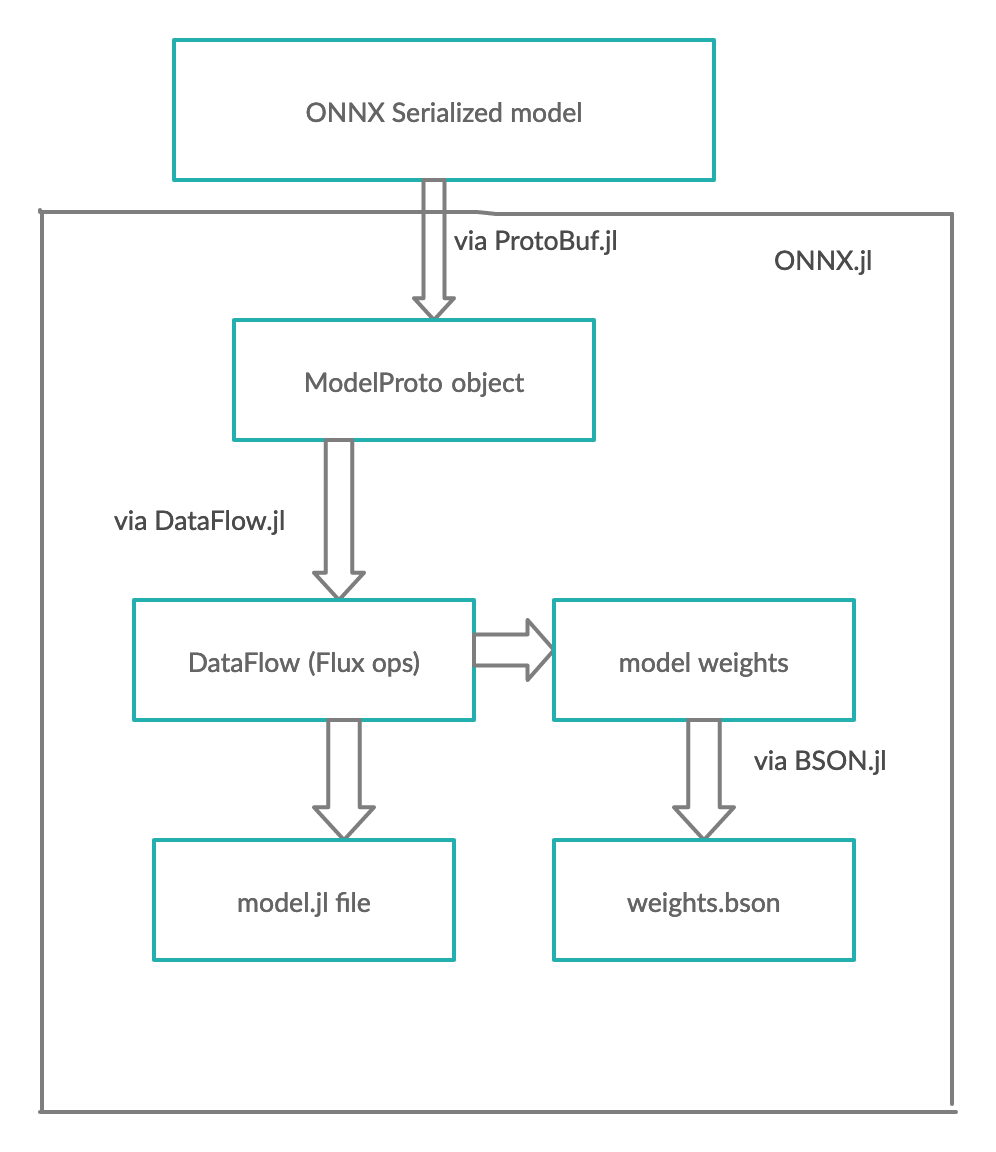
\includegraphics[width=8.8cm]{onnx-3.png}

\begin{center}
    \textit{Fig. 1: Flow diagram of ONNX.jl}    
\end{center}

Additionally, ONNX.jl also provides helper functions for inspecting the model before loading it. \textit{ONNX.layers} reads an ONNX file and returns a list of all the layers in the model. With the growing 
interest around more complicated and deep models, it is possible that an ONNX model might have layers that Flux
itself doesn't support. For handling these, ONNX.jl leaves a \textit{hook} for the users to implement
additional functionality. A \textit{hook} is a function that doesn't have an existing implementation: one
would have to write an implementation for it themselves. However any operator that also has a corresponding
implementation in Flux is completely recognized by ONNX.jl at the moment.

\section{Usage Scenarios}
The ONNX format and ONNX.jl can be used for transfer learning in Flux, where we store knowledge while training a model and
use this knowledge for some other task. The idea is that rather than random initialization of parameters for training a neural network, it's better to take an already trained model, since
it leads to faster convergence. In transfer learning, we take a pretrained model and train it on another 
dataset, which might also have a different class distribution. Fine tuning is an approach to transfer learning
where we train on a subset of training data with a smaller learning rate. Transfer learning learning has shown
tremendous results in image classification, object detection, simulations, sentiment and NLP based classification 
in recent past.    
This is also pretty common when talking about tasks such as neural style transfer where we want to change the 
style of an image in accordance with the style of another image. Generative Adversarial Networks (GANs) have shown
to deliver high quality results when trained on top of a pre-trained model. StyleGAN \cite{DBLP:journals/corr/abs-1812-04948} , for example, can use a
pre-trained model to train a custom model to deliver high quality super-resolution results.

\section{Related Work}

In recent times several projects have come up that solve similar issue. One of the most notable project is
TensorFlow's mlir (Multi-Level Intermediate Representation) \cite{lattner2020mlir} . mlir is an evolution of LLVM 
\cite{LLVM:CGO04} that defines a 
common Intermediate Representation (IR) format, which can be used to represent any DataFlow graph. This common 
format unifies machine learning models in TensorFlow or other frameworks.  
Other noteworthy approaches in this direction are PFA and NNVM. PFA \cite{10.1145/2939672.2939731} or Portable Format for Analytics is a common
language that aims as easing the transition from development to production. It can be expressed within
the common JSON format and has functionalities such as control structures, loops and user-defined functions.
  
NNVM\cite{nnvm} is an end-to-end compiler for AI frameworks. It aims at solving the challenges posed by using different
diverse machine learning frameworks. It consist if two major components: NNVM (Neural Network Virtual Machine)
and TVM (Tensor Virtual Machine) \cite{article} . NNVM defines a common computational graph intermediate representation
format and TVM implements the operators used in these computation graphs while optimizing them for the backend hardware.

\section{Future Work}

As ONNX.jl becomes the beginning point for various researchers interested in using Julia for their research,
it is important to note that it also has certain shortcomings. The most significant is that a model can't
be completely loaded unless there's an equivalent implementation of the operator in Flux.jl. An example of this
is Grouped Convolutions. These variants of Convolutional layers were used in AlexNet \cite{NIPS2012_4824} and showed amazing 
results. However, since Flux doesn't support these at the moment, the users will need to have an implementation
ready if they choose to import an ONNX model with this particular layer into Flux using ONNX.jl. On the plus side,
a lot of the most commonly used layers are available in Flux and can be readily used. Another thing to note is
that to run ONNX.jl generated code in some other hardware, one might need to do a little restructuring. The model
should work directly on the CPU. 

Another challenge moving forward is that we need to constantly update ONNX.jl to support Flux's latest API
changes. This also applies for the other way round: As ONNX operators are updated, we would have to update these
corresponding implementations in ONNX.jl to support the newer models using these updated specifications. Over
the long run, we'd need to constantly keep an eye out for such changes and adapt ONNX.jl to those. Moreover,
there are subtle differences in the way Flux implements operators as compared to other frameworks. As an example,
consider the simple \textit{AveragePool} layer. The way Flux implements this is by padding the input tensor 
appropriately and then performing the pooling operation. However, Keras-tensorflow does this by pooling and then 
padding. This leads to subtle changes along the edges of the tensor in the output. Such differences occur due to
the way most frameworks deal with such layers, and the only way to avoid this is to check for such
discrepancies.

In recent past, DataFlow.jl has been superseded by another intermediate representation format tool: IRTools.jl. 
It provides the ability to work with both lowered and typed Julia code and can be used together with 
metaprogramming tools such as Cassette.jl.  

There has also been some talk about splitting ONNX.jl into two packages: The first one would do the code 
generation and DataFlow related functions while the other would be solely responsible for implementation of the
ONNX operators. This would be greater control and ease while implementing layers or debugging a loaded model. This
should also make implementation pretty straight-forward wherever missing.
For the moment, all this continues to be done by a single package.



\section{Conclusion}

Developing ONNX.jl has been tremendous learning experience. From studying about Intermediate Representation formats for deep 
learning models with millions of parameters to loading them in just a couple of lines of code, ONNX.jl has 
made it very easy and straight-forward to use a high quality trained model as a starting point for many projects.
Once such example I'd like to point out is DenseNet-121 model. This is deep convolutional network that has 
multiple Convolutional, Dense and Pooling blocks. Naturally, implementing this in any framework is going to be
a challenging task. However, thanks to ONNX, we can now use an earlier implementation to import this model into
any other framework. Importing this model (train in Caffe2) via ONNX.jl into Flux can be done in ~3 lines of code.
 

I was also able to load several large computer vision models loaded from ONNX format at the time of actively
developing the package. Most of these have been added to FluxML/Metalhead.jl for a direct plug-and-play use. These
included:

\begin{itemize}
    \item SqueezeNet \cite{i2016squeezenet}
    \item DenseNet 121  \cite{huang2016densely}
    \item ResNet 50     \cite{he2015deep}
    \item GoogleNet     \cite{szegedy2014going}
\end{itemize}


ONNX.jl serves as a entry point for people looking to use Flux for their research, but want quick results. It 
combines the power of the Julia language, the elegance of Flux and the availability of a vast number of pre-trained models. This enables researchers to spend time focusing on the real issues, rather than model portability. \newpage

`% **************GENERATED FILE, DO NOT EDIT**************

\bibliographystyle{juliacon}
\bibliography{ref.bib}


\end{document}

% Inspired by the International Journal of Computer Applications template
